
\begin{frame}{\large Problem Description: Rectification}
\vspace{-0.1in}
\begin{align*}
Z = A\cdot B \pmod{P(X)}
\end{align*}
\vspace{-0.1in}
\begin{figure}[hbt]
\centering
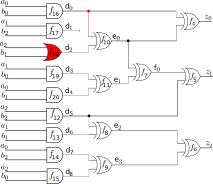
\includegraphics[scale=0.32]{mas_3_sfr.pdf}
\caption*{A buggy implementation of a 3-bit modulo multiplier}
\end{figure}
\end{frame}

\begin{frame}{\large Problem Description: Rectification}
\begin{figure}[hbt]
\centering
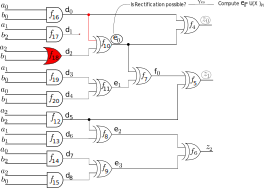
\includegraphics[scale=0.35]{mas_3_sfr2.pdf}
% \caption*{Buggy 2-bit modulo multiplier circuit}
\end{figure}
\end{frame}

\begin{frame}{\large Finite Field Notations}
	\bi
		\item Finite (Galois) Field $\Fq$: 
		\bi
			\item Set of $q$ finitely many elements. $q=p^n$, $p=prime$
		\ei
		\item $\F_2 = \B = \{0,1\}$
		\item On circuits, $p=2$, $n=$ data-operand width 
		\item Hardware cryptography extensively based on $\Fkn$ (we use $\Fkn$)
		\item $\F_2 \subset \Fkn$, $n>1$
		% \item $q = p$ or $q = p^n$ ($k \in \N$); $p$ is a prime
		% \bi
		% 	\item $\F_2$: set of elements 0 and 1
		% 	\item $\F_5$: $\{0,1,2,3,4\}$
		% \ei
		% \item Addition, Multiplication are Associative and Commutative
		% \item $\forall e \in \Fq$ and $e \neq 0$, $\exists e^{-1}$ $s.t. e\cdot e^{-1} = 1$
		% \item Finite (Galois) field $\Fq$ has finitely many elements
		% \item $\F_{p^n}$ ($k \neq 1$) is extension of $\F_p$
		\item Contribution: Application to integer arithmetic circuits
		\bi
			\item Infinite sets: More investigation needed 
		\ei
	\ei
\end{frame}

\begin{frame}{\large Modeling Circuits using Polynomials}
\bi
\item Circuit $C$ modeled as polynomials
\item Boolean logic gates in $\F_2$ ($\F_2 \subset \Fkn$); Over $\F_2$ $-1 = +1 \pmod{2}$)
\begin{align*}
z ~ =  ~ \neg a ~ & \rightarrow ~ z+a+1 \pmod 2  \\
z ~ =  ~ a \wedge b ~ & \rightarrow ~ z+a\cdot b \pmod 2\\
z ~ =  ~ a \vee b ~ & \rightarrow ~ z+a+b+a\cdot b \pmod 2 \\
z ~ =  ~ a \oplus b ~ & \rightarrow ~ z+a+b \pmod 2 
\end{align*}
\item Specification in $\Fkn$, $f_{spec}:Z+AB$
\item Word level polynomials [$\ga=$ Primitive element of $\Fkn$]
\bi
	\item Output: $Z + z_0 +\ga z_1 +\ga^2 z_2 + \cdots +\ga^{n-1} z_{n-1}$,
	\item Input: $A + \sum_{i=0}^{n-1}\ga^ia_i$, and so on
\ei 
\ei
\end{frame}

\begin{frame}{\large Polynomial Ring}
%need to be written in an specific order
%manipulate term-by-term 
\bi
	\item Given $\{x_1,\dots,x_d\}$
	\bi
		\item Monomial $X = x_1^{e_{1}}\cdot x_2^{e_{2}}\cdots x_d^{e_{d}}$, where $e_i \in \Z_{\geq 0}, i\in \{1, \dots,d\}$
		\item Polynomial $f = c_1 X_1 + c_2 X_2 + \dots + c_t X_t$; $c_i \in \Fkn$
	\ei
	\item All such $f$ form the ring $R = \Fkn[x_1,\dots,x_d]$
	% \item Univariate polynomial division, leading term: monomial with highest degree
	\vspace{0.1in}
	\item Multivariate polynomials: need to order the monomials
	\vspace{0.1in}
	\item Impose monomial order ``$>$'' on $R$
	\bi
		\item We utilize \alert{{\it lex}} term order
		% \item lex (for 2 variables, $x_1>x_2$): $x_1^2 >x_1x_2 >x_2^2>x_2>1$ 
	\ei
	\vspace{0.1in}
	\item $f = c_1 X_1 + c_2 X_2 + \dots + c_t X_t$  ~~~(with lex order)
	\bi
		\item $lt(f) = c_1 X_1, ~lm(f) = X_1, ~lc(f) = c_1$
	\ei
\ei
\end{frame}

\begin{frame}{\large Sum, Product, and Quotient of Ideals}
\begin{center}
Given $J_1 = \langle f_1,\dots,f_s\rangle \in R$ and $J_2=\langle h_1,\dots,h_r\rangle \in R$
\end{center}
\bi 
\item Sum of ideals:
\bi
	\item $J_1 + J_2 = \langle f_1,\dots,f_s, h_1\dots,h_r\rangle$
\ei
\item Product of ideals:
\bi
\item $J_1\cdot J_2 = \langle f_i\cdot h_j: 1\leq i\leq s, 1\leq j\leq r\rangle$
\ei

\item Ideal quotient of $J_1$ by $J_2$:
\bi
\item $J_1:J_2 = \{f \in R \ |\ f\cdot h \in J_1, \forall h \in J_2\}$
\ei

\item Ideals and varieties are dual concepts
\bi
\item $V(J_1 + J_2) = V(J_1) \cap V(J_2)$
\item $V(J_1\cdot J_2) = V(J_1) \cup V(J_2)$
\item $V(J_1:J_2) = V(J_1)-V(J_2)$
\ei
% \item Moreover, if $J_1 \subseteq J_2$ then $V(J_1)\supseteq V(J_2)$
\ei

\end{frame}

\begin{frame}{\large Vanishing Ideals} %x^2 - x
% Ensure that var takes values only in $\F_2$
% Boolean values 
\bi
	% \item Fermat's little Theorem: $e \in \Fkk$, $e^{2^k} = e$
	\item For variables in circuit ideals:
	\bi
		\item Bit-level $x_i$: $x_i^2 - x_i$ or $x_i^2 + x_i$ as $-1 = +1\pmod{2}$ over $\Fkn$
		\item Word-level $Z$, $A$: $Z^{2^n} - Z$, $A^{2^n} - A$
	\ei
	\vspace{0.1in}
	\item Vanishing Ideal: $J_0 = \langle F_0 \rangle =  \langle x_1^2+x_1,\dots,x_d^2+x_d, Z^{2^n}+Z, A^{2^n}+A\rangle$
	\vspace{0.1in}
	\item Vanishing Ideal purpose: 
	\bi
		\item Restrict solutions to $x_i$ in $\F_2$
		\item Restrict solutions to $Z,A$ in $\Fkn$
	\ei
	\vspace{0.1in}
	\item For circuits [{\it Lv. et al}, TCAD'13]
	\bi
		% \item vanishing ideals of PIs variables ($\xpi$) required
		\item Only need $\jzpi = \langle \fzpi \rangle = \langle x_i^2 + x_i: x_i \in \xpi \rangle$ added to $J$ 
	\ei
\ei
\end{frame}


\begin{frame}{\large MFR Notations: Composite Field}
\bi
	\item For a given circuit with data-path size $n$
	\bi
		\item Polynomials modeled over $R=\Fkn[Z,A,x_1,\dots,x_d]$
		\bi
			\item $\{x_1, \dots$ $, x_d\}$ are all the bit-level variables (nets) in the circuit
			\item $Z$ and $A$ are the word-level output and input, respectively
		\ei
		\item $\Fkn$ is constructed as $\Fkn = \Ftwo[X]\pmod{P_n(X)}$
		\bi
			\item $P_n(X) \in \F_2[X]$ is a given degree-$n$ primitive polynomial; $P_n(\ga) =0$ 
			% [$\ga$ as one of its root].
		\ei
		\item  The word-level polynomials for $Z,A$ are modeled as:
		\bi
			\item $f_z: Z + \sum_{i=0}^{n-1}\ga^iz_i;f_a: A + \sum_{i=0}^{n-1}\ga^ia_i;$ 
		\ei
	\ei 
	\item Patch $W$ for $m$ targets is computed as a polynomial function in the field $\Fkm$
	\bi
		\item $\Fkm$ is constructed as $\Fkm = \Ftwo[X]\pmod{P_m(X)}$
		\bi
			\item We select a degree-$m$ primitive polynomial $P_m(X)\in \F_2[X]$; $P_m(\be) =0$ 
			% [$\be$ as one of its root].
		\ei
		\item  The word-level polynomial for $W$ is modeled as:
		\bi
			\item $f_w: W + \sum_{i=0}^{m-1}\be^iw_i$
			\item $\{w_0,\dots,w_{m-1}\} \subset \{x_1,\dots,x_d\}$
		\ei
	\ei
\ei
\end{frame}

\begin{frame}{\large MFR Notations: Composite Field}
\bi
	\item Determine the smallest single field ($\Fkk$) to operate both circuit ($\Fkn$) and patch ($\Fkm$)
	\vspace{0.1in}
	\item Smallest $k$ is $LCM(n,m)$
	\bi
		\item $\Fkk \supset \Fkn$ and $\Fkk \supset \Fkm$
		\item $\Fkk$ is constructed as $\Fkk = \Ftwo[X]\pmod{P_k(X)}$
		\bi
			\item $P_k(X)$ is a degree-$k$ primitive polynomial; $P_k(\al) =0$ 
		\ei
	\ei
	\vspace{0.1in}
	\item  Mathematical challenge: Given $P_n(X)$ and $P_m(X)$, compute $P_k(X)$ such that
	$P_n(\ga)= P_m(\be)=P_k(\al)=0$
	\vspace{0.1in}
	\bi
		\item $\ga = \al^{(2^k-1)/(2^n-1)} = \al^{\lambda}$
		\item $\be = \al^{(2^k-1)/(2^m-1)} = \al^{\mu}$
	\ei
	\vspace{0.1in}
	\item Solved using factorization of univariate polynomials over finite fields
\ei

\end{frame}

\begin{frame}{\large MFR Notations: Univariate Polynomial factorization (UPF) }
\bi
	\item Given a monic univariate polynomial $f \in \F_q[X]$, where $\F_q$ is any finite field
	\vspace{0.1in}
	\bi 
		\item Find a complete factorization $f = f_1^{e_1}\cdot f_2^{e_2}\cdots f_l^{e_l}$ 
		\bi
			\item Where $f_1, f_2,\dots, f_l$ are pairwise distinct monic 
			irreducible polynomials in $\F_q[X]$ and $e_1,\dots,e_l$ are positive integers.
		\ei
	\ei
	\vspace{0.1in}
	% \item We employ existing implementation of UPF from computer algebra tool {\it SINGULAR} 
\ei
\end{frame}

\begin{frame}{\large MFR Notations: Finding Primitive Polynomial $P_k(X)$}
\bi
	\item Obtain UPFs of $P_n(X^{\lambda})$ and $P_m(X^{\mu})$
	\bi
		\item Coefficients will be in $\Ftwo$ and degrees will be less than $\lambda$ and $\mu$, respectively.
		\bi
			\item $P_n(X^{\lambda})=P_{n1}^{a1}\cdot P_{n2}^{a2}\cdots P_{nl}^{al}$, and 
			\item $P_m(X^{\mu}) = P_{m1}^{b1}\cdot P_{m2}^{b2}\cdots P_{mg}^{bg}$
		\ei
	\ei
	\vspace{0.1in}
	\item Conjecture: $\exists P_{ni}(X) \in \{P_{n1}, P_{n2},\dots ,P_{nl}\}$ and $\exists P_{mj}(X) \in \{P_{m1}, P_{m2},\dots ,P_{mg}\}$, such that:
	\bi
		\item $P_k(X) = P_{ni}(X)=P_{mj}(X)$,
		\item $P_{k}(X)$ is a degree-$k$ primitive polynomial in $\F_2[X]$ such that $P_k(\al)=0$
	\ei
\ei
\end{frame}


\begin{frame}{\large MFR Application: Verification}
\bi
	\item Circuit designed using irreducible polynomial $P(X) = X^3+X+1$ with $P(\ga)=0$
	\item Denote polynomial $f: Z + A\cdot B$ as the design specification.
	\item Impose RTTO $>$
	\[ \begin{array}{ll}%
f_1:Z + z_0 +\ga z_1 + \ga^2 z_2;   & f_{11}:e_1 + d_3 + d_4; \\       
f_2:A + a_0 +\ga a_1 + \ga^2 a_2;   & \red{f_{12}:d_5 + a_2 + b_2}; \\
f_3:B + b_0 +\ga b_1 + \ga^2 b_2;   & f_{13}:d_6 + a_1b_1; \\          
f_4:z_0 + e_0 + d_0;                & f_{14}:d_7 + a_0b_2; \\          
f_5:z_1 + f_0 + d_5;                & f_{15}:d_8 + a_2b_0; \\          
f_6:z_2 + e_2 + e_3;         & f_{16}:d_0 + a_0b_0; \\
f_7:f_0 + e_0 + e_1;         & f_{17}:d_1 + a_1b_2; \\
f_8:e_2 + d_5 + d_6;         & \red{f_{18}:d_2 + a_2 + b_1 + a_2b_1}; \\
f_9:e_3 + d_7 + d_8;         & f_{19}:d_3 + a_1b_0; \\
\red{f_{10}:e_0 + d_0 + d_2};&    f_{20}:d_4 + a_0b_1;   \\
\end{array}\]%
\ei
\end{frame}

\begin{frame}{\large MFR Application: Verification}
\bi
	\item Polynomial Set
	\bi
		\item $F = \{f_1,\dots,f_{20}\}$ 
		\item $F_0^{PI} = \{a_0^2-a_0, a_1^2-a_1,a_2^2-a_2,b_0^2-b_0, b_1^2-b_1,b_2^2-b_2\}$
	\ei
	\vspace{0.1in}
	\item $f\xrightarrow{F,F_{0}^{PI}}_+= \ga^2(a_2b_2+a_2+b_2)+\ga(a_0b_0+a_1b_2+b_1+a_2b_2+b_2) + (1)(a_0b_0+a_1b_2+b_1+a_2)$
	\vspace{0.1in}
	\item Set of affected outputs: $\Oa = \{z_0,z_1,z_2\}$
	\vspace{0.1in}
	\item Intersection of set of nets in fan-in cones of $\Oa$ is $\emptyset$
	\bi
		\item Implies no SFR points
	\ei
	\vspace{0.1in}
	\item We select $m$=2 and see if the circuit can be rectified by changing
	functions at two nets
\ei
\end{frame}

\begin{frame}{\large MFR Application: Selecting $m$ Targets}
\bi
	\item Since all the outputs are affected, all the nets in the circuit are
	initial candidate targets
	\bi
		\item $\In = \{z_0,z_1,z_2,f_0,e_2,e_3,e_0,e_1,d_5,d_6,d_7,d_8,d_0,d_2,d_3,d_4\}$
		\item Associate a cost for each net driven by synthesis constraints
		\bi
			\item Nets which lie in the intersection of multiple outputs are assigned lowest cost
			\item Rest of the nets are assigned cost based on their topological level in the design
			\item $\Ic = \{4,4,4,3,2,2,-2,2,-2,1,1,1,-2,-2,1,1\}$
		\ei
	\ei
	\vspace{0.1in}
	\item Solved as weighted set cover problem
	\bi 
		\item Partition $\Oa$ into $m$ distinct non-empty subsets such that
		\bi
			\item Intersection of fan-in cones of output bits within a subset is non-empty
		\ei
		\item If such a cover $\M$ exists ($|\M|= m$), each of the $m$ targets are selected from the 
			$m$ distinct covers
		\bi
			\item {\small $\Oa = \{\{z_0,z_1\},\{z_2\}\}$}
			\item {\small $\M = \{\M_0:\{e_0,d_0,d_2\},\M_1:\{d_5,d_6,d_7,d_8,e_2,e_3,z_2\}\}$}
		\ei
	\ei
\ei
\end{frame}


\begin{frame}{\large MFR Application: Word-level Formulation}
\bi
	\item Update ring properties 
	\bi
		\item $R=\F_q[x_1,\dots,x_d,Z,A,W]$
		\item Modify RTTO $>$ to place the target $W$ before the lowest indexed target $e_0$
		\bi
			\item $\{Z\}>\{A>B\}>\{z_0>z_1>z_2\}>\{f_0>e_2>e_3\}>\{{\bf{W}}>e_0>e_1>d_5>d_6>d_7>d_8\}>
				\{d_0>d_1>d_2>d_3>d_4\}>\{a_0>a_1>a_2>b_0>b_1>b_2\}.$
		\ei
	\ei
	\vspace{0.1in}
	\item Update polynomial set $F$ to $F'$:
	\bi
		\item Delete polynomials for $w_i$'s
		\item Delete polynomials in the transitive fan-in of $w_i$'s only
		\item Transitive fan-outs of $w_i$'s need to be replaced with their equivalent 
		word-level representations in terms of $W$
		\item Add $f_w: W + \sum_{i=0}^{m-1}\be^iw_i$
	\ei

\ei
\end{frame}

\begin{frame}{\large MFR Application: Computing $P_k(X)$}
\bi
	\item Composite field: $k=LCM(2,3)=6$
	\vspace{0.1in}
	\bi
		\item $UPF(P_3(X^9)) = \{{\bf X^6+X^4+X^3+X+1},X^6+X^4+X^2+X+1,{\bf X^6+X^5+1}, X^6+X^5+X^2+X+1\}$
		\vspace{0.1in}
		\item $UPF(P_2(X^{21})) = \{{\bf X^6+X^4+X^3+X+1}, {\bf X^6+X^5+1}, X^6+X^3+1, X^6+X^5+X^2+X+1, X^6+X^5+X^3+X^2+1, X^6+X+1, X^6+X^5+X^4+X+1 \}$
		\vspace{0.1in}
		\item We will pick $P_6(X)=X^6+X^4+X^3+X+1$ as the primitive polynomial to setup the unified framework.
	\ei
\ei
\end{frame}

\begin{frame}{\large MFR Notations: Incorrect Primitive Polynomial}
\bi
	\item Note that if we incorrectly choose $P_k(X)=X^6+X^3+1$
	\item For its root $\al$, we have
	\begin{center}
		$\al^6+\al^3+1=0$\\
		$(\al^3)(\al^6+\al^3+1)=0$ (multilying by $\al^3$)\\
		$\al^9+\al^6+\al^3=0$\\
		$\ga+1=0$\label{ga_val}
	\end{center}
	\item But we have $\ga=\al^9$
	\item Selecting arbitrary $P_k(X)$ leads to erroneous results
\ei
\end{frame}

\begin{frame}{\large MFR Application: Word-level Formulation }
\bi
	\item 2-bit rectification patch over the 3-bit circuit can be performed over the field $\F_{2^6}$
	\bi
		\item Field $\F_{2^6} = \F_2[X]$ (mod $P_6(X)$)
	\ei
	\vspace{0.1in}
	\item Update polynomial set $F$ to $F'$ as:
	\begin{center}
		\begin{align*}
			F'=\{f_1,\dots,f_3,f'_4,f'_5,f_6,f'_7,f'_8,f_9,f_w,f_{11},f_{13}\dots,f_{20}\}
		\end{align*}
		{\small\begin{flalign*}
			f'_4:z_0 + (\be W^2 +\be^2 W) + d_0;     &\quad f'_5:z_1 + f_0 + (W^2+W); \\
			f'_7:f_0 + (\be W^2 +\be^2 W) + e_1;   &\quad f'_8:e_2 + (W^2+W) + d_6; \\
			f_w:W + e_0 + \be d_5;             &\quad \be=\al^{21} ; \ga=\al^9;
		\end{flalign*}}
	\end{center}

\ei
\end{frame}

\begin{frame}{\large MFR Contribution: Rectification Check}
%ATPG V() V() = empty
%we have an algebraic proof which is there in the proposal
\bi
	\item Multi-fix rectification at target $W$
	\vspace{0.1in}
	\bi
		\item Construct the following ideals:
		\bi
			\item {\small $J_i = \langle F'_i\rangle =\{f'_1,\dots,f_w=W+\delta(i),\dots,f'_s\}$}
				:$1 \leq i \leq 2^m$, $\delta(0)=0, \delta(1)=1,\delta(2)=\be,\dots,\delta(2^m)= \be^{2^m-2}$
		\ei
		\vspace{0.1in}
		\item Performing the reductions for all $1 \leq i \leq 2^m$: 
		\bi
			\item $f\xrightarrow{F'_i, F_{0}^{PI}}_+r_i $
		\ei
		\item Let $V_{\Fq}(r_i)$ denote the varieties of the respective $r_i$'s
		\vspace{0.1in}
		\item Multi-fix rectification exists at target $W$: \\ 
				\centering
				{\bf if and only if} $\bigcup\limits_{i=1}^{2^m}V_{\Fq}(r_i) = \Fq^{|X_{PI}|} = V(J_0^{PI})$
	\ei
\ei
\end{frame}

\begin{frame}{\large MFR Application: Rectification Check}
\bi
	\item Constructing the $J_i$ ideals:
	\bi
		\item {\small$J_1 = \langle F'_1\rangle$, where $F'_1[f_w]=W+\delta(1)=W$},
		\item {\small$J_2 = \langle F'_2\rangle$, where $F'_2[f_w]=W+\delta(2)=W+1$},
		\item {\small$J_3 = \langle F'_3\rangle$, where $F'_3[f_w]=W+\delta(3)=W+\be$},
		\item {\small$J_4 = \langle F'_4\rangle$, where $F'_4[f_w]=W+\delta(4)=W+\be^2$}
	\ei
	\vspace{0.1in}
	\item Reducing the specification $f: Z+A\cdot B$ modulo these ideals, we get:
	\bi
		\item $r_1 = f \xrightarrow[]{F'_1,F_{0}^{PI}}_+{a_1b_2\ga^3+a_2b_1\ga^3+\ga^4a_2b_2}$
		\item $r_2 = f \xrightarrow[]{F'_2,F_{0}^{PI}}_+{a_1b_2\ga^3+a_2b_1\ga^3+\ga^4a_2b_2+\ga^3}$
		\item $r_3 = f \xrightarrow[]{F'_3,F_{0}^{PI}}_+{a_1b_2\ga^3+a_2b_1\ga^3+\ga^4a_2b_2+\ga^4}$
		\item $r_4 = f \xrightarrow[]{F'_4,F_{0}^{PI}}_+{a_1b_2\ga^3+a_2b_1\ga^3+\ga^4a_2b_2+\ga^6}$
	\ei
	\item Computing $GB(r_1\cdot r_2 \cdot r_3 \cdot r_4, F_{0}^{PI})=F_{0}^{PI}$
	\item Target $W$ with nets $e_0$ and $d_5$ admits MFR
\ei
\end{frame}

\begin{frame}{\large MFR Notation: Computing Rectification Function}
\bi
	\item Compute a rectification function of the form $W = U(X_{PI})$ 
	\bi
		\item Here $U$ is the \textit{unknown component} computed as an $m$-bit-vector word
		\item It represents the function $W = \sum_{i=0}^{m-1}\be^iu_i$ 
		\bi
			\item Where $u_i$'s represent the individual Boolean functions for the respective $w_i$'s.
		\ei
	\ei
	\item The \textit{unknown component} problem is then formulated as an ideal membership test and
	solved using extended \Grobner Basis: 
	\begin{center}
		\begin{align*}
		&W + \be^0 e_0 + \be d_5  = W + U = W +\be^0(a_1b_2+a_2b_1)+\be a_2b_2;\\
		&e_0 = a_1b_2+a_2b_1;~~d_5 = a_2b_2;
		\end{align*}
	\end{center}
\ei
\end{frame}

\begin{frame}{\large Research Objective: Synthesis of Rectification Function}
\bi
	\item Exploring don't cares
	\bi
		\item We computed $U=b_0$, i.e. $f_{10} = e_3 + b_0$
		\item We utilized quotient of ideals to compute alternate corrections
		\bi
			\item ${U^1} = a_1*b_0$
			\item ${U^2} = a_1*b_1*b_0+a_1*b_1+a_1$
		\ei
		\item Polynomial $U$ depends on the polynomial $h_i$ (quotient of division by target $x_i$) 
		\item $h_i$ actually represents the ODCs for the selected target $x_i$
	\ei
	\item Algorithmic computation of rectification polynomials
	\item word-level formulation of don't cares
\ei
\end{frame}



\begin{frame}{\large Research Objective: Integer arithmetic circuits}
\bi
	\item Techniques valid over fields are inapplicable over rings
	\item \Grobner basis and division algorithms are complicated
	\item Can be modeled over $\Q$
	\bi
		\item Rectification function computation can result in {\it fractional coefficients}
		\item Extracting Boolean rectification function requires exhaustive simulation
		\item No scope of optimization as Extended \Grobner basis technique gives zero control
	\ei
\ei

\end{frame}

\begin{frame}{\large Research Objective: Improving Scalability}
\bi
	\item Enhance implementation for finite field circuits:
	\bi
		\item Rectification formulation in terms of internal nets
		\item Address word-level formulation and the mathematical challenges
		\item Devise efficient algorithms based on ZDDs
	\ei
	\vspace{0.2in}
	\item Implementation for Integer arithmetic circuits
	\bi
		\item Bit level reduction technique increases the verification time exponentially
		\bi
			\item No monomial cancellations across output bits
		\ei
		\item Need implicit data structure with a word-level representation
	\ei
	% \item Objective: Compute Boolean polynomials $U_{ON}$, $U_{OFF}$, and $U_{DC}$
	% \bi
	% 	\item Explore don't cares from quotient of division
	% 	\item Formulate as reductions in $\F_2$
	% 	\item Use ZDDs for the computations
	% \ei
	% \item $J_L + \jzpi$ contains:
	% \bi
	% 	\item Miter Polynomial, $f_m : t(Z-Z_S)-1 = tZ-tZ_S-1$ 
	% 	\item Specification Polynomial, $f_{spec} : Z_S + \mathcal{F}(A)$
	% 	\item $Z+\sum_{i=0}^{k-1}z_i\alpha^i,~ A + \sum_{i=0}^{k-1}a_i\alpha^i$, and so on.
	% 	\item Polynomials from logic gates except $f_i$
	% 	\item Vanishing polynomials $x_i^2 + x_i: x_i \in \xpi$
	% \ei
\ei
\end{frame}

% \begin{frame}
% \bi
% 		\item Application to ECOs and Approximate circuits
% 		\bi
% 			\item Current circuit implementation should be minimally 
% 			modified (rectified) to match the ECO-evolved/approximate specification
% 		\ei
% \ei
% \end{frame}